\documentclass[convert]{standalone}

\usepackage{tikz}
\usepackage{graphicx}
\pagestyle{empty}

% INT_AY22_L28-Fig12_Cube.png

\begin{document}
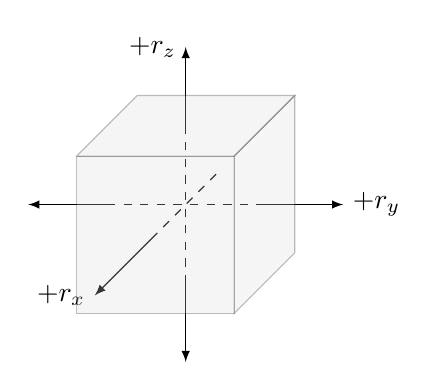
\begin{tikzpicture}[> = latex, every node/.style = {color = black, opaque}]

	% Definition
	
	\def\S{1}		% Scaling size used for object

	% In the given coordinate system, z points out of the page while y points towards
	% the top of the page. I flipped these two coordinate systems, so we are looking
	% at the object from the side.

	% Coordinate axes
	
	\begin{scope}[dashed]
	
		\draw (-\S, 0, 0) -- (\S, 0, 0);
		\draw (0, -\S, 0) -- (0, \S, 0);
		\draw (0, 0, -\S) -- (0, 0, \S);
	
	\end{scope}
	
	\begin{scope}[->]
	
		\draw (\S, 0, 0) -- (2, 0, 0) node [right] {$+r_y$};
		\draw (0, \S, 0) -- (0, 2, 0) node [left] {$+r_z$};
		\draw (0, 0, \S) -- (0, 0, 3) node [left] {$+r_x$};
	
		\draw (-\S, 0, 0) -- (-2, 0, 0);
		\draw (0, -\S, 0) -- (0, -2, 0);
	
	\end{scope}
	
	% Cubic gaussian surface
	
	\draw [fill = gray!30, nearly transparent] (\S, \S, \S) -- (-\S, \S, \S) -- (-\S, -\S, \S) -- (\S, -\S, \S) -- cycle;
	\draw [fill = gray!30, nearly transparent] (\S, \S, \S) -- (\S, -\S, \S) -- (\S, -\S, -\S) -- (\S, \S, -\S) -- cycle;
	\draw [fill = gray!30, nearly transparent] (\S, \S, \S) -- (-\S, \S, \S) -- (-\S, \S, -\S) -- (\S, \S, -\S) -- cycle;
	
\end{tikzpicture}
\end{document}